
% Die 'book' Klasse sorgt für die gewünschte Formatierung, 
% Kapitel, \frontmatter, \mainmatter, etc.
\documentclass[a4paper,oneside,openright,11pt]{book}

% --- Kernpakete ---
\usepackage[T1]{fontenc}
\usepackage{lmodern} % Schriftart Latin Modern
\usepackage[utf8]{inputenc}
\usepackage[ngerman]{babel} % Für deutsche Silbentrennung und Begriffe
\usepackage{parskip}
\usepackage{graphicx} % Für Bilder (Logo)


% --- Nützliche Pakete aus Ihrer Vorlage ---
\usepackage{listings} % Für Code-Blöcke (Dockerfile, etc.)
\usepackage{amssymb}
\usepackage{amsmath}
\usepackage{url}
\def\UrlBreaks{\do\/\do-} % Zeilenumbrüche in URLs
\usepackage{hyperref} % Klickbare Links (Inhaltsverzeichnis, URLs)
\usepackage{xspace}
\usepackage{csquotes}
\usepackage{rotating}

%  Unser eigenes Titel-Paket
\usepackage{tikz}
\usetikzlibrary{positioning}

\usepackage{projectdoc} 

\MakeOuterQuote{"}
% 
% Vermeidet "Overfull \hbox" (Text ragt über den Rand)
\setlength{\emergencystretch}{3em}
\hyphenpenalty=5000
\tolerance=1000

% --- HIER ALLE TITELSEITEN-DATEN EINGEBEN ---

% 1. Logo (muss im selben Ordner liegen)
% WICHTIG: Kommentieren Sie diese Zeile aus, wenn die Logo-Datei nicht existiert
\unilogo{
\includegraphics[scale=1]{FHDW-Logo.eps}} 

% 2. Uni-Name (optional, kann leer bleiben)
\uniname{}

% 3. Dokumententyp
\docType{Projektdokumentation} 

% 4. Projektname (Haupttitel)
\title{19th Century London Data}

% 5. Version
%\version{Version 1.0}

% 6. Autoren (mit \and trennen)
\author{Leonie Abels, Amirreza Ahmadi Darani, Aziz Klebleyev, Bjarne Möller, \and Franz Müller, Xuan-Loc Tran}


% 7. Kurs / Modul
\course{Data Analytics}

% 8. Professor
\prof{Prof. Dr. Jil Klünder}

% 9. Datum
\date{\today}

% --- Ende der Daten ---

\begin{document}

% --- VORDERTEIL (Frontmatter) ---
% Sorgt für römische Seitenzahlen (i, ii, iii...)
% und keine Kapitelnummern im Inhaltsverzeichnis
\frontmatter

% Erstellt die Titelseite
\maketitle

% Optional: Fügen Sie hier eine Management Summary ein
% \chapter*{Management Summary}
% Hier kommt Ihre Zusammenfassung...
% \clearpage

% Erstellt das Inhaltsverzeichnis
\chapter*{Selbstständigkeitserklärung}
Hiermit versichern wir, dass wir den Projektbericht ``Miniprojekt Teil 1, Dokumentation der Phasen 1--3'' selbständig verfasst und keine anderen als die angegebenen Quellen verwendet haben.
Alle Textstellen und andere Inhalte wie Bilder, Quellcode oder Daten, die direkt, wörtlich oder sinngemäß aus anderen Quellen entnommen sind, haben wir eindeutig mit korrekten Quellenangaben versehen.

\tableofcontents

% --- HAUPTTEIL (Mainmatter) ---
% Startet die Seitenzählung bei 1, 2, 3...
% Kapitel werden jetzt nummeriert
\mainmatter

% Wir laden den Inhalt für jedes Kapitel aus dem Ordner 'kapitel/'
% Dies hält Ihre Hauptdatei sauber und übersichtlich.

\chapter{Einleitung und Fragestellung}
\label{chap:einleitung}

Die vorliegende Dokumentation beschreibt die Durchführung und die Ergebnisse unseres Datenanalyseprojekts im Rahmen des Moduls Data-Analytics.
Gemäß der im Kurs behandelten Phasen liegt der Fokus auf der Definition einer Fragestellung,
der methodischen Datenbeschaffung sowie der Anwendung moderner statistischer Verfahren zur Ableitung von Handlungsempfehlungen.

\section*{Armut im viktorianischen London}
\label{sec:kontext}
Während des 19.\ Jahrhunderts versuchte der Positivist Charles Booth, Ausmaß und Ursachen der Armut in East-London zu erfassen.
Dafür nutzte er bestehende statistische Daten,
die er dann analysierte, kategorisierte, und schließlich 1897 in \textit{"LIFE AND LABOUR OF THE PEOPLE IN LONDON"}\ (im Folgenden auch als \textit{"LIFE AND LABOUR"} abgekürzt)
\cite{life_and_labour} veröffentlichte,
welches eines der bekanntesten Exemplare einer frühen (vor-) soziologischen Studie ist.

Dafür führt er die in \autoref{tab:booth_classes} beschriebene Klassifikation der Arbeiterklasse ein.

\begin{table}[htbp]
\centering
\caption{Charles Booths Klassifikation sozialer Schichten}
\label{tab:booth_classes}

\begin{tabular}{|c|p{4.8cm}|c|p{3.8cm}|}
\hline
\textbf{Class} & \textbf{Description} & \textbf{Category} & \textbf{Alias} \\
\hline

A & Lowest class &
very poor \& semi-criminal &
Lowest Class \\
\hline

B & Casual earnings &
very poor \& semi-criminal &
Casual Earnings \\
\hline

C & Intermittent earnings &
poor &
Irregular Earnings \\
\hline

D & Small regular earnings &
poor &
Regular Minimum \\
\hline

E & Regular standard earnings &
comfortable &
Ordinary Earnings \\
\hline

F & Higher class labour &
comfortable &
Highly Paid Work \\
\hline

G & Lower middle class &
well to do &
Lower Middle \\
\hline

H & Upper middle class &
well to do &
Upper Middle \\
\hline

\end{tabular}
\end{table}

\section*{Motivation und Relevanz}
In der Entstehungsgeschichte der Soziologie sind Armut und Ungleichheit neben Religion, und Angewohnheiten und Verhalten zentrale Themen.
Es ging dabei häufig darum, den Ausmaß von Armut im Zuge der Industriellen Revolution und seiner Folgen zu Messen.
Auch in modernen Gesellschaften sind Armut und Ungleichheit weit verbreitet, wenn auch nicht im selben Ausmaß.
Nichtsdestotrotz bietet der Blick auf die Zeit, in der unsere modernen Gesellschaften entstanden eine wertvolle Perspektive.

Dafür werden in dieser Arbeit mögliche Faktoren für Armut und die Entstehung sozialer Ungleichheit untersucht.

\subsection*{Methodische Motivation: Moderne Analyse historischer Daten}
Da Charles Booth in seiner Zeit keinen Zugang zu modernen statistischen Methoden und Tests hatte, ist auch interessant,
inwiefern wir mit diesen neue Einsichten erlangen können.
Insbesondere ist auch eine grafische Aufbereitung der Daten, die über die Bar-Charts in \textit{"LIFE AND LABOUR"} hinausgeht möglich.

\section*{Verfeinerung der Fragestellung}
\label{sec:verfeinerung}

Unsere ursprüngliche Fragestellung lautet: \textit{„Welche Faktoren bestimmten die Armut im London des 19. Jahrhunderts?“}.

\subsection*{Konkretisierung und Hypothesenbildung}
Um die Fragestellung operabel zu machen, haben wir sie in drei konkrete Untersuchungsebene unterteilt:

\begin{figure}[h]
    \centering
    \begin{tikzpicture}[
        scale=0.9,
        transform shape,
        scale=0.8,
        transform shape,
        node distance=2.8cm and 2.8cm,
        every node/.style={font=\small},
        main/.style={
            rectangle,
            rounded corners,
            draw=black,
            thick,
            align=center,
            minimum width=4.8cm,
            minimum height=1.2cm,
            fill=gray!10
        },
        sub/.style={
            rectangle,
            rounded corners,
            draw=black,
            align=center,
            text width=4.8cm,
            minimum height=3.6cm,
            fill=blue!5
        },
        arrow/.style={
            ->,
            thick
        }
    ]

    % main node
    \node[main] (poverty)
    {\textbf{Armut im viktorianischen London}};

    % sub node
    \node[sub, below left=of poverty] (demo)
    {
        \textbf{Demografisches Risiko}\\[0.2cm]
        Haushaltsgröße\\
        Anteil der Kinder\\[0.3cm]
        \scriptsize
        Welchen Einfluss hat die Haushaltsgröße,\\
        insbesondere der Anteil der Kinder,\\
        auf die Zugehörigkeit zur Armutsklasse?
    };

    \node[sub, below=of poverty] (struct)
    {
        \textbf{Strukturelles Risiko}\\[0.2cm]
        Berufsstatus\\
        Sektion / Tätigkeit\\[0.3cm]
        \scriptsize
        Inwieweit ist der Berufsstatus\\
        ein isolierter Prädiktor für Armut,\\
        wenn demografische Faktoren kontrolliert werden?
    };

    \node[sub, below right=of poverty] (social)
    {
        \textbf{Soziales Risiko}\\[0.2cm]
        Familienstand\\
        Witwer / Alleinstehende\\[0.3cm]
        \scriptsize
        Besteht ein signifikanter Zusammenhang\\
        zwischen Familienstand und extremer Armut?
    };

    % arrowssssssss
    \draw[arrow] (demo) -- (poverty);
    \draw[arrow] (struct) -- (poverty);
    \draw[arrow] (social) -- (poverty);

    \end{tikzpicture}

    \caption{Grafische Verfeinerung der Fragestellung gemäß Phase 1}
    \label{fig:fragestellung}
\end{figure}

\chapter{Methodik}
\label{chap:methodik}

In diesem Kapitel wird der Prozess der Datenakquise und -aufbereitung detailliert beschrieben. Da für die Fragestellung keine modernen digitalen Datensätze zur Verfügung standen, musste eine Brücke zwischen historischer Dokumentation und moderner Datenanalyse geschlagen werden.

\section*{Beschreibung der Datenquelle}
Als primäre Datenquelle dient das Werk \textit{"Life and Labour of the People in London"} von Charles Booth (1886--1903). Die Analyse stützt sich auf die detaillierten Tabellen, in denen die Bevölkerung Londons nach Berufsfeldern (section*s) und sozialen Klassen (A--H) kategorisiert wurde. Jede Zeile der Originaltabellen enthält Informationen über:
\begin{itemize}
    \item Die \textbf{Berufsklasse} (z. B. Labour, Artisans, Dealers).
    \item Demografische Merkmale wie \textbf{Heads of Families}, \textbf{Wives} und \textbf{Children} unter 15 Jahren.
    \item Die Verteilung der Personen auf die \textbf{sozialen Klassen A bis H}.
\end{itemize}

\section*{Problematik unklarer oder ungenauer Daten}
Der Datensatz beruht auf den gesammelten Daten von 'School Board Visitors' die Hausbesuche bei Familien mit Kindern im Schulalter und 2-3 Jahre vor dem Schulalter machten und den Beruf des Familienhaupts festhielten. Die Menge der in diesem Datensatz erfassten Menschen beläuft sich auf die Hälfte der Bevölkerung der beschriebenen Distrikte und ist davon ausgehend hochgerechnet.
Booth macht zunächst einige grundlegende Annahmen:
Er geht davon aus, dass Schulkinder in der Regel ältere und jüngere Geschwister haben und schätzt auf die gezählte Anzahl der Schulkinder, noch einmal die selbe Menge von Geschwisterkindern ("Children and young persons 13-20") zu den selben Klassen und Berufsgruppen hinzu.
Auch geht er davon aus, dass die verheirateten Männer verschiedener Klassen und Berufsgruppen mit Schulkindern generell repräsentativ sind für verheiratete Männer derselben Klasse und Beruf ohne Schulkinder, mit der Begründungen, sie würden ihren Beruf wählen bevor sie Kinder im Schulalter haben und auch nachdem die Kinder nicht mehr in der Schule sind weiterhin in diesem Beruf tätig sind.

Diese Schätzungen beinhalten keinerlei Überlegung, dass gerade ärmere Familien sich möglicherweise gegen (weitere) Kinder entschieden, da sie sich keine (weiteren) Kinder leisten konnten.
Abtreibungen waren in England seid 1803 illegal (Malicious Shooting or Stabbing Act 1803), doch Abtreibungsmittel wurden trotzdem großflächig in Frauenmagazinen beworben, mit vagen oder blumigen Umschreibungen als "Catholic Pills", "Womans Helper" oder auch als Abführmittel. Der Rückgang der Geburtenrate in Großbritannien von 35.5/1000 in den 1870ern zu 29/1000 in 1900, unterstützt die Interpretation, dass Frauen in der UK in diesem Zeitraum, die ihnen zur Verfügung stehenden Mittel nutzten um Schwangerschaften zu planen.

Es lässt sich anmerken, dass Booths gelieferten Daten teils ungenau sind. So werden an einigen Stellen Schätzungen vorgenommen, die nicht als solche ausgezeichnet sind. Da sich in den Datensätzen Werte befinden die offensichtlich Abschätzungen sind, wie z.B. eine Menge an exakt 40.000 Menschen in einer Kategorie.

Auch sind manche Formulierungen für uns heute nicht mehr nachvollziehbar. Was genau die Benennung einer Gruppe damals beinhaltet hat, ob es eine allgemein bekannte Definition gab usw.

Trotz all diesen Einwänden und Schätzungen, die Menge der erhobenen Daten ist mit 50\% der Bevölkerung der erfassten Stadtteile ein wertvoller Einblick in die damaligen Bevölkerungsstrukturen und vertretenen Berufsgruppen in London.

\section*{Datenerhebung und manuelle Transkription}
Die Datenerhebung erfolgte durch die manuelle Übertragung der Informationen aus digitalen Scans der Originalseiten in ein maschinenlesbares Format (CSV). Dieser Prozess umfasste:
\begin{itemize}
    \item \textbf{Digitalisierung:} Übertragung der gedruckten Tabellen in CSV-Dateien für jeden untersuchten Borough.
    \item \textbf{Qualitätssicherung:} Abgleich der übertragenen Werte mit den Originalwerten zur Vermeidung von Übertragungsfehlern.
    \item \textbf{Umgang mit historischen Begriffen:} Beibehaltung der originalen Bezeichnungen, um die historische Authentizität zu wahren.
\end{itemize}


\section*{Eingesetzte Tools und Infrastruktur}
Für die Verwaltung und Verarbeitung der Daten wurden folgende Werkzeuge genutzt:
\begin{itemize}
    \item \textbf{GitHub:} Versionskontrolle und Zusammenarbeit im Team. Die Nutzung von Branches (z. B. \texttt{trial}-Branch) ermöglichte eine parallele Bearbeitung von Skripten und Datensätzen.
    \item \textbf{Python (Pandas):} Zentrale Bibliothek für die Datenmanipulation. Pandas wurde gewählt, da es eine effiziente Harmonisierung unterschiedlicher Tabellenstrukturen und eine automatisierte Berechnung neuer Metriken ermöglicht.
\end{itemize}

\section*{Vorgehen bei der Datenzusammenführung (Data Merging)}
Ein entscheidender Schritt war die Kombination der einzelnen Distrikt-Tabellen zu einem Gesamtdatensatz (\texttt{merged\_london\_data.csv}). Das Vorgehen gliederte sich in:
\begin{enumerate}
    \item \textbf{Standardisierung:} Vereinheitlichung der Spaltennamen, da die Originalscans teilweise leicht variierende Schreibweisen (z. B. "Heads of Famlies" vs. "Heads of Families") aufwiesen.
    \item \textbf{Konkatenation:} Zusammenführung der Daten aus den Boroughs Bethnal, Green, Hackney, Mile End Old Town, Poplar, Shoreditch, Stepney und St. George's-in-the-East.
    \item \textbf{Aggregatbildung:} Integration der Zusammenfassungen auf Borough-Ebene (\texttt{classes\_boroughs\_total.csv}) und Berufsebene (\texttt{professions\_total.csv}) zur Validierung der Gesamtsummen.
\end{enumerate}
\chapter{Datenverarbeitung und Vorverarbeitung }
\label{chap:vorverarbeitung}

In dieser Phase wurden die digitalisierten Rohdaten bereinigt und transformiert, um eine präzise Beantwortung der Forschungsfragen zu ermöglichen. Ein wesentlicher Bestandteil war die Überprüfung statistischer Voraussetzungen, um die Belastbarkeit der späteren Modelle sicherzustellen.

\section*{Datenbereinigung / Data Cleaning}
Bevor die eigentliche Analyse beginnen konnte, mussten die aggregierten Daten aus den verschiedenen Boroughs harmonisiert werden.
\begin{itemize}
    \item \textbf{Standardisierung:} Spaltenbezeichnungen wurden vereinheitlicht, um Inkonsistenzen zwischen den Teildatensätzen zu beseitigen. Dies umfasst z.b. die Korrektur von "Heads of Famlies" zu "Heads of Families".
    \item \textbf{Umgang mit Fehlwerten:} Da leere Felder in den historischen Tabellen oft das Nichtvorhandensein einer Gruppe signalisierten, wurden \textit{NaN}-Werte (Not-a-Number) durch Nullen ersetzt, um mathematische Berechnungen zu ermöglichen.
    \item \textbf{Deskriptive Vorstudie:} Es wurde eine deskriptive Statistik durchgeführt, um ein Gefühl für die Verteilungen und mögliche "Ausreißer-Berufe" zu erhalten.
\end{itemize}

Hieraus ließ sich folgender Boxplot für die Armutsraten erstellen:

\begin{figure}[htbp!]
    \centering
    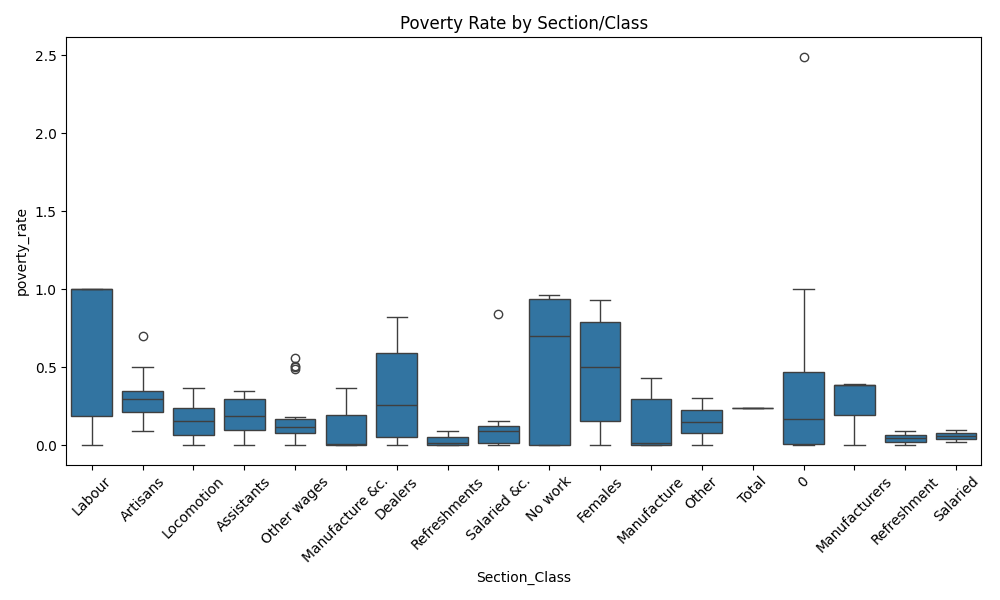
\includegraphics[width=1.2\textwidth]{contents/figures/boxplot_poverty_rate.png}
    \caption{Boxplot Armutsklassen}
    \label{fig:povertyClasses}
\end{figure}

\section*{Feature Engineering: Konstruktion von Metriken}
Um die Fragestellung nach Risikofaktoren operationalisierbar zu machen, wurden aus den Rohdaten neue Variablen berechnet:
\begin{itemize}
    \item \textbf{Poverty Rate:} Um die Armut messbar zu machen, wurde die Quote der Klassen A bis D im Verhältnis zur Gesamtbevölkerung einer Sektion berechnet: 
    \[ poverty\_rate = \frac{A + B + C + D}{Total} \]
    \item \textbf{Kids per Household:} Um die demografische Belastung zu erfassen, wurde die Anzahl der Kinder pro Haushaltsvorstand ermittelt (\textit{Children / Heads of Families}).
\end{itemize}

\section*{Statistische Voraussetzungsprüfung}
Ein zentraler Aspekt der Qualitätssicherung war die Überprüfung der Normalverteilung. 
\begin{itemize}
    \item \textbf{Shapiro-Wilk-Test:} Der Test auf die \textit{poverty\_rate} ergab eine Test-Statistik von 0,8229 und einen p-Wert von $9,11 \times 10^{-19}$.
    \item \textbf{Ergebnis:} Da der p-Wert weit unter der Schwelle von 0,05 liegt, wurde die Nullhypothese einer Normalverteilung abgelehnt. Die Stichprobe ist somit nicht-gaussisch (not Gaussian).
\end{itemize}

\section*{Methodische Konsequenzen}
Aufgrund der fehlenden Normalverteilung wurden die Analysepläne angepasst, um die Validität der Ergebnisse nicht zu gefährden:
\begin{itemize}
    \item \textbf{Nicht-parametrische Tests:} Für Gruppenvergleiche wurde der Kruskal-Wallis-Test anstelle einer ANOVA gewählt.
    \item \textbf{Korrelationen:} Die Zusammenhänge wurden mittels Spearman-Rangkorrelation anstelle von Pearson untersucht. Grund ist, dass die Spearman-Rangkorrelation robust gegenüber nicht-normalverteilten Daten ist.
    \item \textbf{Modell-Anpassung:} Für die Regression wurde ein transformiertes Modell (Log-Transformation) in Betracht gezogen, um die Residuen-Eigenschaften zu verbessern.
\end{itemize}

\begin{figure}[htbp!]
    \centering
    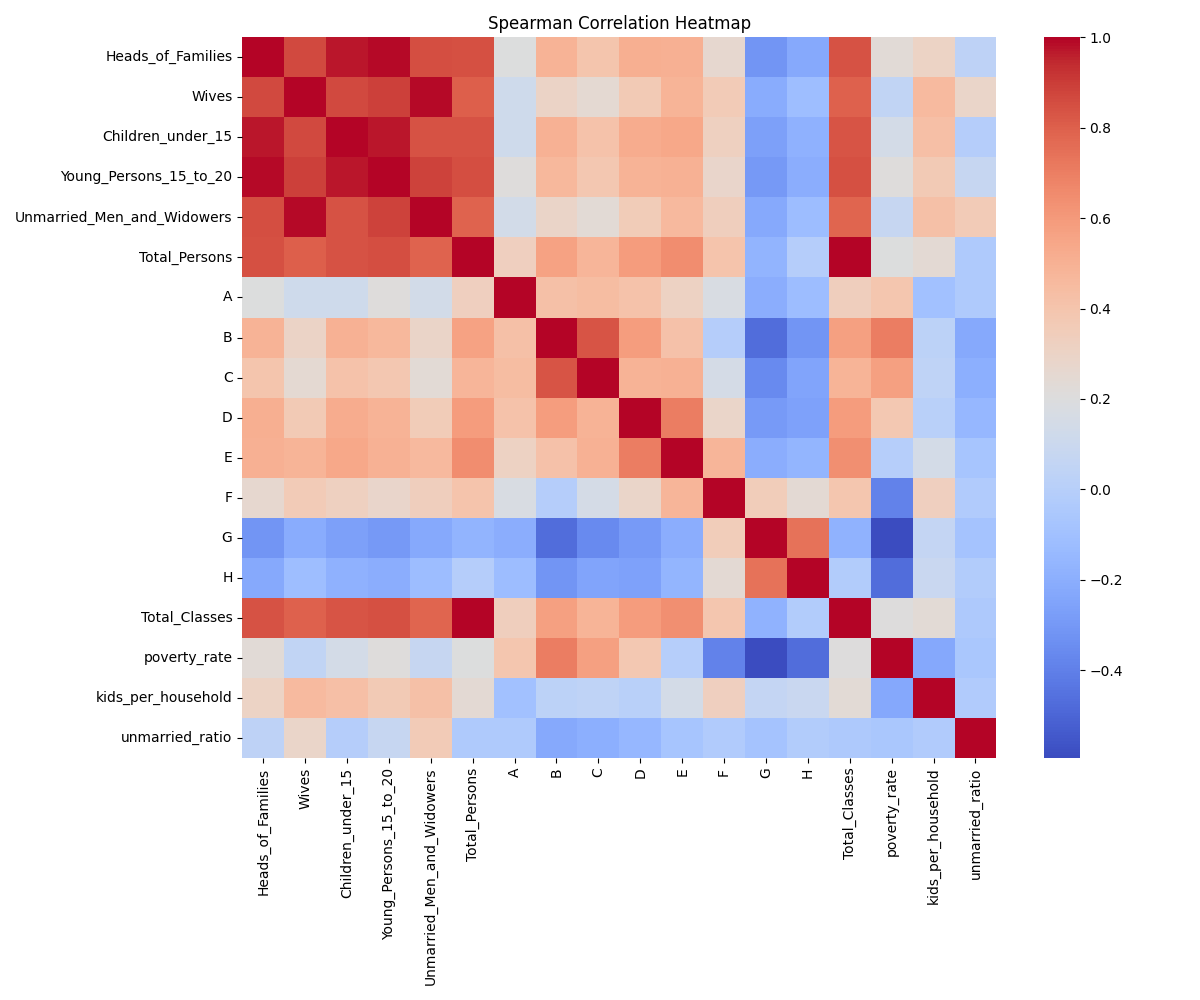
\includegraphics[width=0.85\textwidth]{contents/figures/correlation_heatmap.png}
    \caption{spearman correlation}
    \label{fig:spearman correlation}
\end{figure}
\chapter{Datenanalyse und Modellbildung}
\label{chap:analyse}

In dieser Phase erfolgte die tiefergehende Untersuchung der Forschungsfrage nach den Risikofaktoren für Armut. Basierend auf den Erkenntnissen der Vorverarbeitung wurden nicht-parametrische Tests für Gruppenvergleiche und  multivariate Regressionsmodelle eingesetzt.

\section{Explorative Analyse der Berufsgruppen}
Um festzustellen, ob sich das Armutsrisiko zwischen den verschiedenen sozialen Sektionen signifikant unterscheidet, wurde ein Gruppenvergleich durchgeführt. Da die Voraussetzung der Normalverteilung verletzt war, wurde der \textbf{Kruskal-Wallis-Test} als nicht-parametrische Alternative zur ANOVA gewählt.

\begin{itemize}
    \item \textbf{Ergebnis:} Der Test lieferte eine Teststatistik von $H = 68,15$ bei einem p-Wert von $4,47 \times 10^{-08}$.
    \item \textbf{Interpretation:} Die Nullhypothese, dass die Armutsrate über alle Sektionen hinweg gleich verteilt ist, wurde abgelehnt. Es existieren somit hochsignifikante Unterschiede im Armutsrisiko zwischen den Berufsgruppen.
\end{itemize}

\section{Multivariate Modellierung der Risikofaktoren}
Um den Einfluss mehrerer Faktoren gleichzeitig zu isolieren, wurde eine multiple lineare Regression (OLS) berechnet. Hierbei wurden zwei Modelle verglichen, um die bestmögliche statistische Güte zu erreichen.

\subsubsection{Modellvergleich und Residuendiagnostik}
Ein zentrales Gütekriterium für Regressionsmodelle ist die Normalverteilung der Residuen.
\begin{itemize}
    \item \textbf{Basis-Modell:} Die Residuen des ursprünglichen Modells wiesen eine starke Abweichung von der Normalverteilung auf ($p = 4,59 \times 10^{-10}$).
    \item \textbf{Transformiertes Modell:} Durch eine Log-Transformation ($\log1p$) der Zielvariable \textit{poverty\_rate} konnte die Verteilung der Residuen signifikant verbessert werden (Teststatistik: 0,9842; $p = 0,001$).
\end{itemize}
Aufgrund dieser Ergebnisse wurde das transformierte Modell für die finale Interpretation gewählt, da es die statistischen Voraussetzungen besser erfüllt.

\subsubsection{Robustheit der Schätzung}
Um die Ergebnisse jenseits rein deskriptiver Zahlen abzusichern, wurde die Kovarianz-Matrix des Modells mit \textbf{robusten Standardfehlern (Typ HC3)} berechnet. Dieses Verfahren schützt die Signifikanztests vor Verzerrungen durch Heteroskedastizität, was angesichts der historischen Datenqualität eine notwendige methodische Absicherung darstellt.

\subsubsection{Zusammenfassung der Modellergebnisse}
Das finale Modell erreicht ein bereinigtes Bestimmtheitsmaß ($Adj. R^{2}$) von $0,192$. Dies bedeutet, dass ca. $19,2\%$ der Varianz der Armutsrate durch die einbezogenen Faktoren erklärt werden können. Sämtliche Koeffizienten wurden auf ihre Signifikanz geprüft, um belastbare Aussagen über die Risikofaktoren treffen zu können.

\begin{figure}[htpb!]
    \centering
    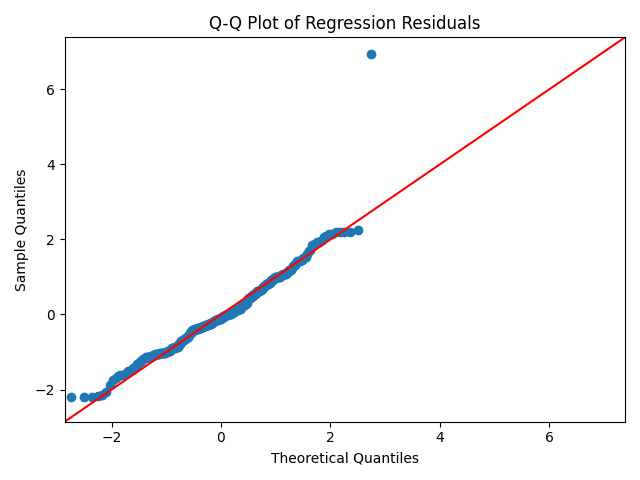
\includegraphics[width=0.65\textwidth]{contents/figures/regression_qqplot.png}
    \caption{regression-qqplot}
    \label{fig:regression1}
\end{figure}

\begin{figure}[htpb!]
    \centering
    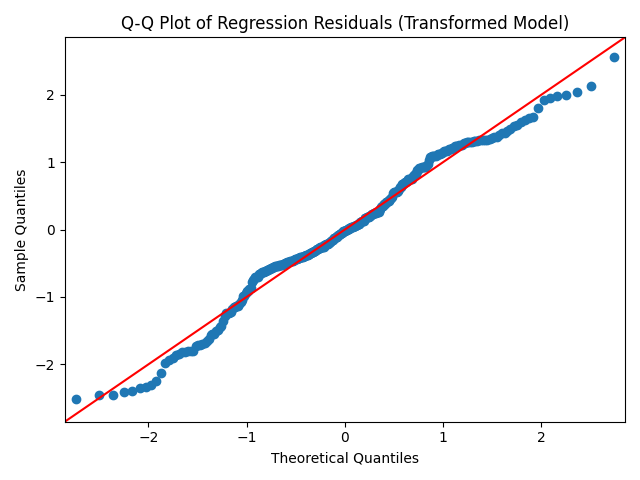
\includegraphics[width=1.1\textwidth]{contents/figures/transformed_model_qqplot.png}
    \caption{regression-qqplot2}
    \label{fig:regression3}
\end{figure}

\chapter{Ergebnisse und Interpretation}
\label{chap:ergebnisse}

In diesem Kapitel werden die Ergebnisse der statistischen Modellierung präsentiert und im Hinblick auf die Forschungsfrage nach den Risikofaktoren für Armut interpretiert. Die Analyse basiert auf dem transformierten Regressionsmodell mit robusten Standardfehlern (HC3), welches die höchste statistische Belastbarkeit aufweist.

\section*{Identifikation zentraler Risikofaktoren}
Die Regressionsanalyse identifiziert zwei primäre strukturelle Risikofaktoren, die einen signifikanten positiven Einfluss auf die Armutsrate haben:

\begin{itemize}
    \item \textbf{Berufsstatus "`Labour"':} Mit einem Koeffizienten von $0,2339$ ($p < 0,001$) stellt die Zugehörigkeit zur Gruppe der unqualifizierten Tagelöhner das größte Armutsrisiko dar. Dies bestätigt Booths deskriptive Beobachtungen auf mathematischer Ebene.
    \item \textbf{Weibliche Haushaltsvorstände:} Sektionen mit einem hohen Anteil an weiblichen Vorständen weisen einen signifikanten Koeffizienten von $0,1583$ ($p = 0,004$) auf. Dies deutet darauf hin, dass Haushalte ohne männlichen Verdiener (oft bedingt durch Arbeitsunfälle oder Verwitwung) im viktorianischen London besonders vulnerabel waren.
\end{itemize}

\section*{Schutzfaktoren und soziale Stabilität}
Im Gegensatz dazu konnten deutliche Schutzfaktoren identifiziert werden, die mit einer signifikanten Verringerung der Armutsrate korrelieren:
\begin{itemize}
    \item Berufe im Sektor \textbf{Salaried} (Angestellte) sowie im Bereich \textbf{Refreshments} (Gastgewerbe) weisen stark negative Koeffizienten auf (z. B. $-0,2185$, $p < 0,001$). Regelmäßige Einkommen und eine feste Anstellung waren somit die effektivsten Mittel zur Armutsprävention.
\end{itemize}

\section*{Demografie vs. Struktur}
Ein wesentliches Finding der Analyse ist die fehlende Signifikanz der demografischen Variablen im multiplen Modell:
\begin{itemize}
    \item \textbf{Kinderzahl:} Entgegen der ursprünglichen Hypothese liefert die Variable \textit{kids\_per\_household} ($p = 0,414$) keinen signifikanten zusätzlichen Erklärungsbeitrag zur Armutsrate, sobald der Berufsstatus kontrolliert wird.
    \item \textbf{Alleinstehende Männer:} Auch das \textit{unmarried\_ratio} ($p = 0,359$) ist statistisch nicht signifikant.
\end{itemize}
Dies deutet darauf hin, dass Armut im 19. Jahrhundert primär ein \textbf{strukturelles Problem des Arbeitsmarktes} und weniger ein rein demografisches Problem der Haushaltsgröße war.

\section*{Güte und Belastbarkeit des Modells}
Das Modell erklärt ca. $23,8\,\%$ der Varianz der Armutsrate ($R^{2} = 0,238$). Während dies für sozialwissenschaftliche Daten ein solider Wert ist, bleibt ein Großteil der Varianz durch Faktoren ungeklärt, die nicht in den historischen Tabellen erfasst wurden, z.b. individuelle Gesundheitszustände oder lokale Mietpreise. Es muss zudem kritisch angemerkt werden, dass es sich um \textbf{Korrelationen}, nicht zwingend um Kausalitäten handelt. 
\chapter{Anwendung des Modells und Handlungsempfehlungen}
\label{ch:handlungsempfehlungen}
\section*{Tagelöhner}
Neben keiner Arbeit scheint auch Arbeit als Tagelöhner ein signifikantes Risiko für Armut zu sein.
Unser Modell beschreibt, dass eine Gesellschaft, in der ungesicherte Arbeitsverhältnisse weit verbreitet sind, viel Armut und Ungleichheit aufweist.
Nachdem die starken Gewerkschaften des 20.\ Jahrhunderts in den letzten 40 Jahren stark an Bedeutung verloren haben, sehen
wir heute einen starken Shift zur sog.\ Gig-Economy, die eine moderne Ausprägung von Tagesarbeit darstellen könnte.
Sollten diese Trends andauern, lässt sich mit unserem Modell ein wachsendes Armutsproblem prognostizieren.

Allerdings ist wichtig anzumerken, dass diese Prognose auf einem Modell einer geschichtlichen Gesellschaft beruht.
Somit beschränkt sich der Vergleich an dieser Stelle auf die qualitative Ebene,
inwiefern ein Schluss von damals auf heute möglich ist, lässt sich nicht quantifizieren.

\section*{Frauen}
In unserem Modell sind Frauen als Familienoberhaupt stärker von Armut gefährdet als Familien mit Männern als Familienoberhaupt.
Zwar lässt sich hier eine parallele zu den durchschnittlich geringeren Einkommen von Frauen in der heutigen Gesellschaft vermuten,
unserer Ansicht nach ist die höhere Armutsrate an dieser Stelle jedoch insbesondere der Form der erhobenen Daten geschuldet.
So sind Frauen nur als Familienoberhaupt (also als Haupteinkommensquelle der Familie) vermerkt, wenn kein Mann älter als 20 Jahre in diesem Haushalt lebt.
Wir sehen somit nicht unbedingt den Unterschied zwischen Einkommen von Männern und Frauen, sondern hauptsächlich, dass Haushalte mit maximal einem Einkommen
eine höhere Armutsrate aufweisen als solche mit einem oder mehr Einkommen, was zu erwarten ist.
Wir können somit keine Aussage über den Stand von Frauen in der Arbeitswelt und der Gesellschaft im viktorianischen London treffen.



% % --- ANHANG (Appendix) ---
\appendix % Schaltet hier auf Anhang-Kapitel um (Kapitel A, B, C...)

\appendix % Schaltet auf den Anhang-Modus um (A, B, C...)

\chapter{Appendix}

\begin{table}[h]
\centering
\caption{OLS Regression Results}
\label{tab:ols_results}

\scriptsize

\begin{tabular}{|l|r|r|r|r|}
\hline
\textbf{Variable} & \textbf{Coef.} & \textbf{Std. Err.} & \textbf{z} & \textbf{P$>|z|$} \\
\hline

Intercept & 0.2497 & 0.059 & 4.231 & 0.000 \\
Artisans & 0.0116 & 0.034 & 0.344 & 0.731 \\
Assistants & -0.0791 & 0.051 & -1.552 & 0.121 \\
Dealers & 0.0126 & 0.055 & 0.229 & 0.819 \\
Females & 0.1583 & 0.055 & 2.877 & 0.004 \\
Labour & 0.2339 & 0.066 & 3.558 & 0.000 \\
Locomotion & -0.0943 & 0.043 & -2.177 & 0.029 \\
Manufacture & -0.1222 & 0.060 & -2.035 & 0.042 \\
Manufacture \&c. & -0.1393 & 0.068 & -2.037 & 0.042 \\
Manufacturers & -0.0232 & 0.144 & -0.161 & 0.872 \\
No work & 0.1001 & 0.102 & 0.986 & 0.324 \\
Other & -0.1176 & 0.196 & -0.600 & 0.548 \\
Other wages & -0.0908 & 0.046 & -1.955 & 0.051 \\
Refreshment & -0.2003 & 0.048 & -4.201 & 0.000 \\
Refreshments & -0.2185 & 0.032 & -6.746 & 0.000 \\
Salaried & -0.1898 & 0.042 & -4.526 & 0.000 \\
Salaried \&c. & -0.1398 & 0.049 & -2.872 & 0.004 \\
Total & -0.0166 & 1.152 & -0.014 & 0.988 \\
kids\_per\_household & -0.0220 & 0.027 & -0.817 & 0.414 \\
unmarried\_ratio & 0.4120 & 0.449 & 0.917 & 0.359 \\
\hline
\end{tabular}

\vspace{0.3cm}

\begin{tabular}{|l|r|}
\hline
\textbf{Model Information} & \textbf{Value} \\
\hline
Dependent Variable & log\_poverty\_rate \\
R-squared & 0.238 \\
Adjusted R-squared & 0.192 \\
F-statistic & 16.67 \\
Prob (F-statistic) & $5.42 \times 10^{-37}$ \\
No. Observations & 331 \\
Df Residuals & 311 \\
Df Model & 19 \\
Covariance Type & HC3 \\
Durbin-Watson & 1.651 \\
Jarque-Bera (JB) & 15.796 \\
Prob (JB) & 0.000371 \\
Cond. No. & 63.9 \\
\hline
\end{tabular}

\vspace{0.3cm}

\footnotesize
\textit{Notes: Standard Errors are heteroscedasticity robust (HC3).}

\end{table}


\begin{table}[h]
\centering
\caption{Statistical Test Results}
\label{tab:statistical_tests}

\small

\begin{tabular}{|p{6cm}|c|c|p{4.5cm}|}
\hline
\textbf{Test} & \textbf{Statistic} & \textbf{p-value} & \textbf{Conclusion} \\
\hline

Shapiro-Wilk Test for Normality on poverty\_rate
& 0.8229
& $9.1119 \times 10^{-19}$
& The sample does not look Gaussian (reject $H_0$)
\\
\hline

Kruskal-Wallis Test on poverty\_rate across Section\_Class
& 68.1526
& $4.4751 \times 10^{-8}$
& Significant difference between sections (reject $H_0$)
\\
\hline

Shapiro-Wilk Test for Normality on Regression Residuals (Base Model)
& 0.9423
& $4.5952 \times 10^{-10}$
& Residuals do not look Gaussian (reject $H_0$)
\\
\hline

Shapiro-Wilk Test for Normality on Regression Residuals (Transformed Model)
& 0.9842
& $1.0606 \times 10^{-3}$
& Residuals do not look Gaussian (reject $H_0$)
\\
\hline

\end{tabular}

\vspace{0.4cm}

\footnotesize
\textbf{Model Comparison:}
The transformed model using $\log(1+x)$ better fulfills the statistical prerequisites, particularly the normality assumption of residuals.

\end{table}
     

% --- RÜCKTEIL (Backmatter) ---
% ( Bibliografie, die wir brauchen!!!!)
\backmatter

\end{document}
